\chapter{Materiais e Métodos}
\label{chap:mat}
Esta seção destaca o que é necessário para construção do projeto, contendo a lista de materiais, especificação dos componentes, funcionalidades, modelo esquemático de comunicação e de alimentação.

%--------- NEW SECTION----------------------
\section{Especificação dos componentes}
\label{sec:espc}
Serão detalhados os componentes utilizados para confecção do protótipo, sendo eles físicos ou digitais.

\subsection{Estrutura analítica do protótipo}
\label{ssec:pbs}


\subsection{Lista de componentes}
\label{ssec:list}

\subsection{Servomotores}
Os servomotores são responsáveis pelo atuação do robô, realizando os movimentos das juntas dos braços e das garras, além de atuarem as rodas que deslocam o robô na linha. São utilizados os servomotores da Robotis, \textit{Dynamixel} MX-106R e MX-28. Esses motores foram escolhidos pois apresentam drivers prontos para o \textit{ROS} , que possibilitam uma integração mais fácil com as ferramentas de controle, apresentando bom torque, peso reduzido e fácil integração para controle conjunto.


\begin{table}[]
	\begin{tabular}{ll}
		
		\multicolumn{2}{c}{Robotis Dynamixel MX-28R}                                            \\ \hline
		Peso (g)                     & 153                                                      \\ \hline
		Dimensões (mm)               & 40.2 x 65.1 x 46                                         \\ \hline
		Torque (N.m)                 & 8.0 (em 11.1V), 8.4 (em 12V) e 10.0 (em 14.4V)           \\ \hline
		Temperatura de operação (ºC) & -5 até +80                                               \\ \hline
		Tensão de operação (V)       & 10 até 14.8 (Tensão recomendada: 12V)                    \\ \hline
		Baud rate                    & 8000bps até 4.5Mbps                                      \\ \hline
		Protocolo de comunicação     & RS485                                                    \\ \hline
		Resolução                    & 0.088º                                                   \\ \hline
		ID                           & 254 ID (0 até 253)                                       \\ \hline
		Feedback                     & Posição, temperatura, carga, tensão de alimentação, etc. \\ \hline
	\end{tabular}
\end{table}

 

\begin{figure}[h!]												
	\centering												
	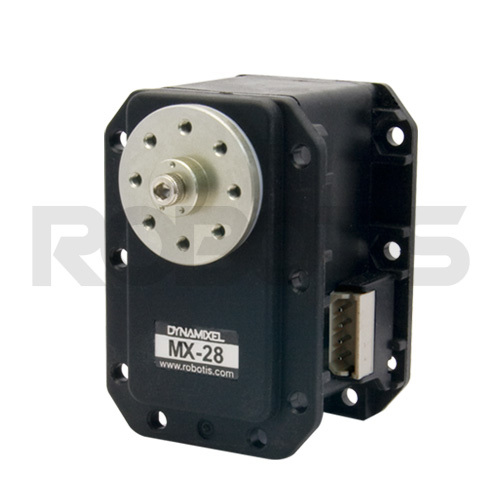
\includegraphics[width=0.32\textwidth]{mx-28r.jpg}				
	\caption{Motor Robotis\textit{ Dynamixel} MX-106R.}		
	\label{img:ihelic}												
\end{figure}
\hspace{2cm}
\begin{table}[]
	\begin{tabular}{ll}
	
		\multicolumn{2}{c}{Robotis Dynamixel MX-28R}                                            \\ \hline
		Peso (g)                     & 153                                                      \\ \hline
		Dimensões (mm)               & 40.2 x 65.1 x 46                                         \\ \hline
		Torque (N.m)                 & 8.0 (em 11.1V), 8.4 (em 12V) e 10.0 (em 14.4V)           \\ \hline
		Temperatura de operação (ºC) & -5 até +80                                               \\ \hline
		Tensão de operação (V)       & 10 até 14.8 (Tensão recomendada: 12V)                    \\ \hline
		Baud rate                    & 8000bps até 4.5Mbps                                      \\ \hline
		Protocolo de comunicação     & RS485                                                    \\ \hline
		Resolução                    & 0.088º                                                   \\ \hline
		ID                           & 254 ID (0 até 253)                                       \\ \hline
		Feedback                     & Posição, temperatura, carga, tensão de alimentação, etc. \\ \hline
	\end{tabular}
\end{table}
\hspace{1cm}

\begin{figure}[h!]												
	\centering												
	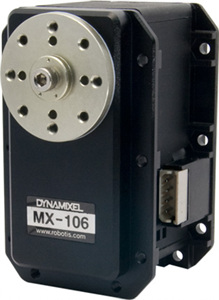
\includegraphics[width=0.2\textwidth]{mx-106r.jpg}				
	\caption{Motor Robotis\textit{ Dynamixel} MX-106R}		
	\label{img:ihelic}	
	
\end{figure}
\subsection{Placa de Gerenciamento de Energia (Power Management)}
A placa de gerenciamento de energia é responsável pela distribuição de corrente e de tensão para todos os componentes elétricos e eletrônicos do robô, além de monitorar os níveis de tensão e corrente demandados durante a operação. 

Além de realizar o monitoramento do consumo em cada porta individualmente, a placa possui um sistema de proteção, cortando a alimentação em casos de surto de corrente. A placa funciona através da alimentação de 14.4 Volts provenientes da placa multiplexadora, responsável por transmitir a carga de duas baterias \textit{Li-Íon} de 14.4 Volts e 6Ah.

Na placa de \textit{Power Management} existem conversores DC/DC responsáveis por fazer a conversão dos níveis de 14.4 Volts para 12 Volts em cada porta de saída da placa. As 7 portas de saída  possuem sensores de tensão e corrente individuais, feitos com amplificadores de instrumentação INA226. Existem duas portas de saída que disponibilizam tensões em valores menores, de 5 Volts. 

O monitoramento dos níveis de tensão e corrente se dá principalmente pela inteligência do sistema, um firmware embarcado em um microcontrolador Atmega32u4, responsável por fazer as leituras dos parâmetros em cada uma das portas, verificando se os seus níveis estão de acordo com os limites configurados, cortando a alimentação via relés digitais caso esses valores sejam ultrapassados.

\subsection{\textit{ROS} (Robot Operating System)}
\textit{Framework}, no ambiente de programação, é um espaço onde compatibiliza códigos comuns a fim de otimizar o trabalho e tempo, muito utilizado na área de desenvolvimento. A abstração de hardware, códigos de baixo nível, drivers de sensores, simuladores, etc - são as grandes vantagens de se utilizar essa aplicação, podendo assim,fazer com que o desenvolvedor foque somente nas soluções de problemas específicos do seu projeto.

Foi utilizado durante todo o desenvolvimento do \textit{ELIR} o \textit{framework} \textit{ROS}, já que reúne uma série de ferramentas importantes para o desenvolvimento de um robô. Como colocado no site oficial do \textit{ROS} temos que o Sistema Operacional de Robótica é um flexível \textit{framework} para escrita de softwares para robótica. É uma coleção de ferramentas, bibliotecas e convenções que serve para simplificar a tarefa de criar complexos e robustos comportamentos de robôs diante a uma variedade de plataformas. 

A grosso modo, cada câmera, motor ou periférico ligado ao \textit{ROS}, estão associados ao um nó. A comunicação entre os nós se dá através de tópicos ou de serviços, a diferença é que o primeiro a informação é trocada de forma constante com certo intervalo de tempo e o segundo somente quando solicitado.

Assim é feita toda a comunicação e interligação entre os periféricos no \textit{ROS}, forma simples de integração dos componentes.

\subsection{\textit{MoveIt!}}
Durante a inspeção de linha, é necessário que o robô realize a ultrapassem dos diferentes tipos de obstáculos que existem nas linhas de transmissão. O \textit{MoveIt!} é um ferramenta que funciona de forma integrada com o \textit{ROS}, apresentando funcionalidades de planejamento de movimento, percepção 3D,controle , manipulação e cinemática inversa. 

A cinemática é o estudo do movimento, no âmbito da robótica designa o estudo do controle da posição do robô no espaço. Esse controle pode representar do robô como um todo, sua posição geográfica, ou controle de alguma parte sua em específico, como seu braço e a posição relativa desse braço e o robô.  A cinemática direta é o cálculo onde se encontra a posição do robô para determinado valor de velocidade ou posição de suas juntas. Analogamente, na cinemática inversa, se encontra os valores de velocidade ou posição das juntas para uma posição no espaço,onde essa posição é denominada \textit{end-effector}, geralmente sendo definido como a parte do robô que interage com o mundo, como por exemplo a garra no caso de manipuladores. O cálculo da cinemática inversa envolve equações complexas e retorna diferentes soluções, assim sendo necessário encontrar a solução que melhor atende às diretrizes do movimento, o \textit{MoveIt!} já realiza esse cálculo e fornece uma trajetória otimizada baseada em parâmetros do usuário.

Outra das suas vantagens é utilizar o modelo \textit{URDF} do robô. \textit{URDF} é uma sigla para Unified Robot Description Format, e designa um arquivo com extensão \verb|.urdf| e sintaxe em XML. É um dos tipos de modelos mais utilizados na robótica atual,sendo escolhido pois apresenta uma sintaxe simples e dinâmica, proporcionando conversões em outros formatos de forma fácil. Define o robô como um conjunto de partes, chamadas de \textit{links} onde a união entre essas partes é uma junta. Onde cada \textit{link} vai ter um \textit{link} pai, que é determinado pela definição da junta, assim o modelo apresenta uma estrutura em árvore, onde todos os \textit{links} vão ter um pai até chegar ao \textit{link} da raíz,essa definição é importante pois a partir disso é feita a cinemática inversa do robô. Um erro no modelo \textit{URDF} acarreta em uma mudança no comando que é mandado para o robô original.

Durante o desenvolvimento do projeto, foi possível realizar a integração do \textit{MoveIt!} com o robô real, sendo possível realizar movimentos físicos utilizando a ferramenta de visualização para posicionamento de end-effector pelo usuário. Porém, ao tentar se enviar um comando com o valor de posição para o end-effector se mover, o programa falhou em encontrar soluções para a cinemática. Mesmo se utilizando os diversos solucionadores providos e enviando valores possíveis de se calcular, o programa sempre estava falhando em encontrar uma solução.

O \textit{MoveIt!} é designado para funcionar com robôs de 6 graus de liberdade, onde cada grau de liberdade indica uma coordenada que o end-effector pode se mover e um dos 3 eixos de referência (x,y,z) que ele pode girar. A grande quantidade de graus de liberdade faz com que os solucionadores utilizem formas de cálculos complexas, assim robôs que possuem menos que 6 graus de liberdade precisam ser compatibilizados, já que a solução leva em consideração todas as direções e giros. O Elir possuI somente 2 graus de liberdade, e as soluções que antes funcionavam não estavam se utilizando especificamente da solução de cinemática inversa provida pelo \textit{MoveIt!}. Assim, decidiu-se realizar o cálculo da cinemática inversa por meio de um código python, que utiliza a equação de cinemática inversa específica para o tipo de braço do robô e fornece os ângulos de junta necessários para o end-effector especificado. 

Com o ângulo de junta em mãos, é feita a integração do robô com a ferramenta, de forma que o planejamento de movimento ocorre, só que com o software recebendo um ângulo desejado. Conhecendo os possíveis valores de end-effector, o que pode ser encontrado pela ferramenta de visualização, é possível realizar o movimento no robô enviando somente um comando de coordenadas.

Implementar o controle de movimento nessa plataforma possibilita uma série de implementações futuras que aumentam a autonomia do robô e robustez do sistema, como odometria, ferramentas de percepção e mapeamento.

\subsection{\textit{Gazebo}}
O software \textit{Gazebo} é software utilizado para simulação de robôs. Tem uma licença de uso livre e apresenta diversas formas de integração com o \textit{ROS}, sendo o principal simulador utilizado em conjunto com essa plataforma, possibilitando a inserção de plugins como câmeras e sonares, que se comunicam com o \textit{ROS} de forma fiel a dispositivos reais.

Nele é possível simular também o ambiente do robô, definindo parâmetros físicos como aceleração da gravidade e vento. Oferece suporte para a inserção de modelos 3D de softwares CAD, assim podendo ser inseridas diversas estruturas que já foram modeladas para outros propósitos no software.

\subsection{\textit{Visual Studio Code}}
Para que todas as funcionalidades do robô sejam configuradas e desenvolvidas de forma correta a nível de software, é necessário o desenvolvimento de diversos códigos em diferentes linguagens para a configuração de aspectos específicos do projeto.

Foi utilizada durante o desenvolvimento do projeto a ferramenta \textit{Visual Studio Code}. Trata-se de um editor de códigos open source desenvolvido pela \textit{Microsoft} em 2015, sendo possível desenvolver códigos em diversas linguagens como C++, C, Python entre outros. Durante todo o desenvolvimento do \textit{ELIR} a ferramenta fora utilizada para o desenvolvimento de arquivos nas extensões .py, .yaml, .launch e .urdf.  

Por ter uma interface simples e amigável, o \textit{VSCode} mostrou-se uma ferramenta extremamente útil para a escrita e desenvolvimento de códigos durante todas as fases do projeto. 

\subsection{\textit{PlatformIO}}
Na interface do \textit{} existem diversas extensões que podem ser instaladas para adicionar novas funcionalidades na plataforma.

Uma das extensões utilizadas fora o \textit{PlatformIO}, um ecossistema desenvolvido especificamente para o desenvolvimento de códigos e firmwares em plataformas microcontroladas, sendo extremamente versátil, tendo suporte para diversas plataformas como STM, MSP430, Arduino entre outras, tornando desnecessário o uso de uma IDE específica para se realizar a configuração e desenvolvimento de firmwares durante o projeto.

A necessidade de se utilizar essa extensão se deu principalmente pela necessidade de se embarcar o firmware da Power Management na placa. O \textit{PlatformIO} possui as funcionalidades de debug e gravação, sendo assim, todos os procedimentos necessários para atualizar o firmware são atendidos na extensão.


%--------- NEW SECTION ----------------------
\section{Diagramas mecânicos}
\label{sec:diagm}


%--------- NEW SECTION ----------------------
\section{Modelo esquemático de alimentação e comunicação}
\label{sec:modesq}


\subsection{Diagramas elétricos}
\label{sec:diage}
Devido à quantidade de motores presentes no robô e a forma com que eles estão distribuídos na estrutura, foram desenvolvidos dois modelos de hubs para a conexão dos motores na rede.

\begin{figure}[h!]												
	\centering												
	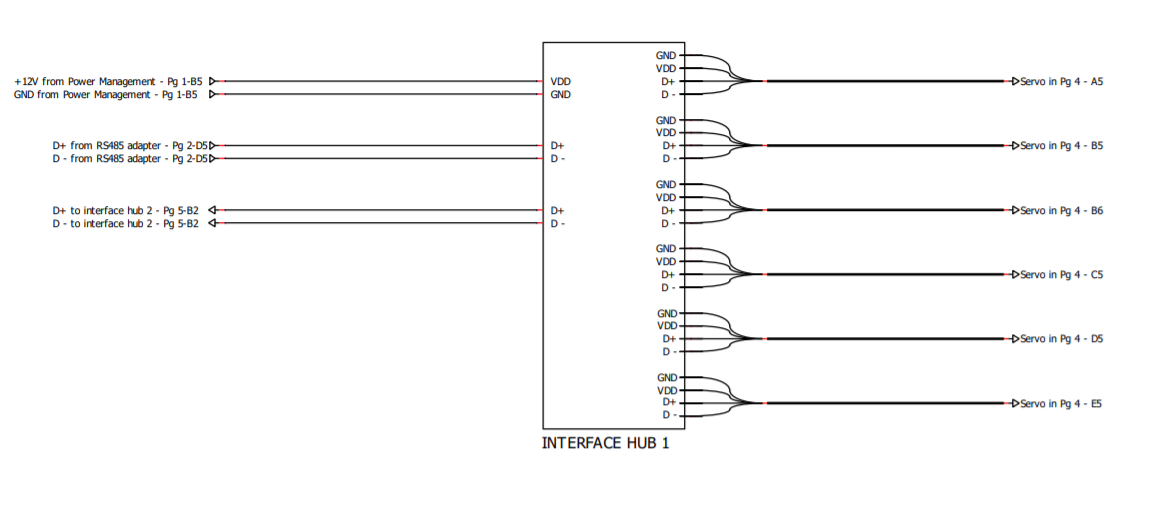
\includegraphics[width=0.4\textwidth]{esquema_hub.png}				
	\caption{Esquema HUB.}		
	\label{img:hub1}									
\end{figure}

\begin{figure}[h!]												
	\centering												
	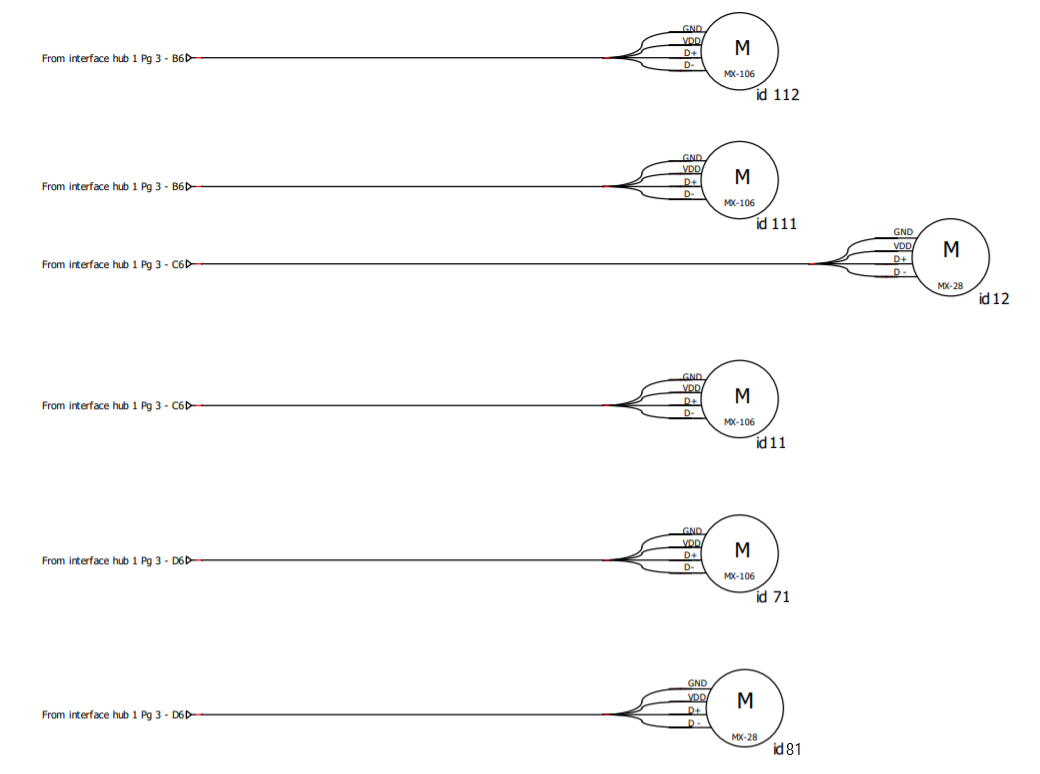
\includegraphics[width=0.4\textwidth]{esquema_hub2.PNG}				
	\caption{Esquema HUB2.}		
	\label{img:hub2}									
\end{figure}

\subsection{Esquemas eletrônicos}
\label{ssec:esqe}
Nas unidades de tração do robô, os hubs contam com um conector de alimentação, um para a entrada de dados e 6 de saída para os motores.
IMAGEM
\begin{figure}[h!]												
	\centering												
	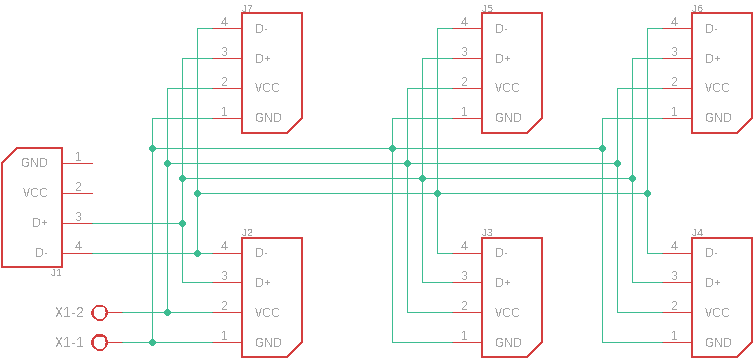
\includegraphics[width=0.3\textwidth]{hub_arm_SCHEMATIC.png}				
	\caption{Esquema HUB2.}		
	\label{img:hub2}									
\end{figure}

\begin{figure}[h!]												
	\centering												
	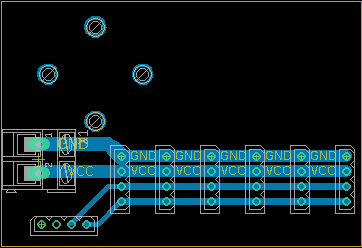
\includegraphics[width=0.3\textwidth]{hub_arm_BOARD.png}				
	\caption{Esquema HUB2.}		
	\label{img:hub2}									
\end{figure}

Já na unidade central, o hub além de conectar os seis motores ali presentes, também é responsável pela conexão dos hubs das unidades de tração e do conversor rs485 que está ligado à \textit{NUC}.
\begin{figure}[h!]												
	\centering												
	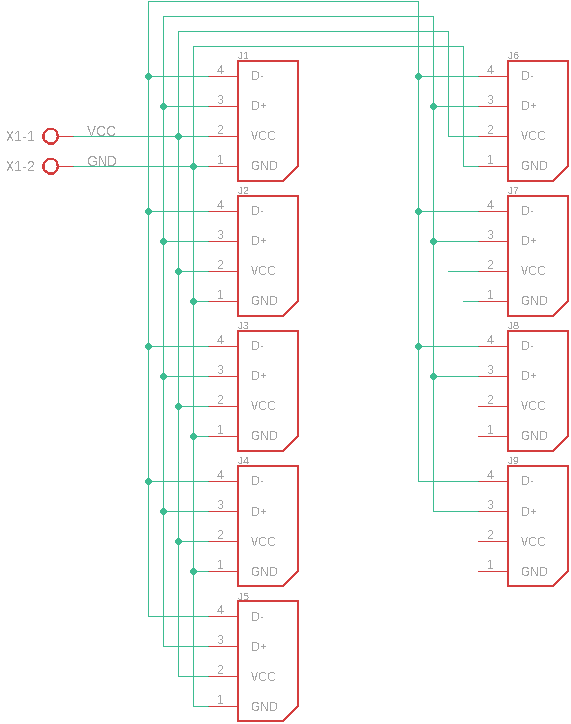
\includegraphics[width=0.3\textwidth]{hub_central_SCHEMATIC.png}				
	\caption{Esquema HUB2.}		
	\label{img:hub2}									
\end{figure}

\begin{figure}[h!]												
	\centering												
	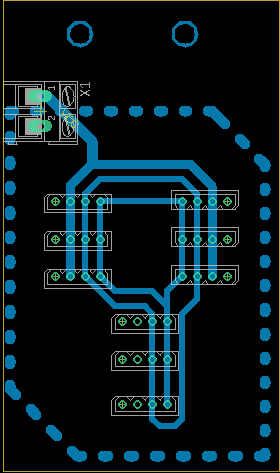
\includegraphics[width=0.3\textwidth]{hub_central_BOARD.png}				
	\caption{Esquema HUB2.}		
	\label{img:hub2}									
\end{figure}

%--------- NEW SECTION ----------------------
\section{Especificação das funcionalidades}
\label{sec:espf}


\subsection{Fluxo das informações}
\label{ssec:fluxo}


\subsection{Motion Planning}
\label{ssec:motion}
\subsubsection{Definição da funcionalidade}
A funcionalidade de \textit{Motion Planning} é responsável por realizar o planejamento da trajetória do Robô, utilizando o software \textit{MoveIt!} que realiza o cálculo da cinemática inversa para encontrar a melhor forma de ultrapassar os obstáculos.
\subsubsection{Dependências}
O software \textit{MoveIT!} pode utilizar o modelo matemático da cinemática inversa do robô ou um arquivo do tipo \textit{URDF}.
O nome \textit{URDF} é uma sigla para \textit{Unified Robot Description Format}, esse arquivo é uma especificação em \verb|XML| utilizada para descrever robôs. Modelos em \textit{URDF} apresentam uma simplicidade na descrição do robô, e para o caso do Robô \textit{Elir}, utilizar o modelo \textit{URDF} possibilitará uma aproximação fiel ao modelo real do robô, assim para o cálculo da cinemática inversa será utilizado o seu modelo \textit{URDF} e não o seu modelo matemático.

\subsubsection{Premissas Necessárias}
Para o correto funcionamento dessa funcionalidade as seguintes premissas são necessárias:
\begin{itemize}
	\item A configuração dos limites de giro das juntas do robô estarão compatíveis com os comandos enviados
	\item O modelo \textit{URDF} do robô estará adequado com o modelo físico
	\item O pacote gerado pelo \textit{MoveIt! Setup Assistant} estará configurado adequadamente
\end{itemize}
\subsubsection{Descrição da Funcionalidade}
A movimentação do robô na linha acontecerá por movimentos de translação e transposição de obstáculos. A translação na linha será feita por controladores de torque nas rodas do robô, enquanto a transposição do obstáculos utilizará o \textit{MoveIT!}.
Por meio da ferramenta \textit{MoveIt! Setup Assistant}, se utiliza o modelo do robô para criar um pacote do \textit{ROS} com os principais arquivos pelo \textit{MoveIT!}. 
A configuração correta do \textit{MoveIT!} possibilita que se utilizem as funções da sua biblioteca para o cálculo da trajetória, levando em consideração também obstáculos no caminho.

O \textit{MoveIT!} fornece uma \textit{user interface} que recebe o end-effector,a nomenclatura atribuída ao node feito em python que recebe o \textit{end-effector} é \verb|moveit_commander|. O  \textit{node} responsável por fazer a integração da user interface com os parâmetros recebidos pelo \textit{ROS Parameter Server} com o \textit{end-effector} para fazer os cálculos é denominado \verb|move_group|. O \textit{node} \verb|move_group| também pode receber parâmetros como leituras dos sensores do robô e nuvens de pontos.

\begin{figure}[H]
	\centering
	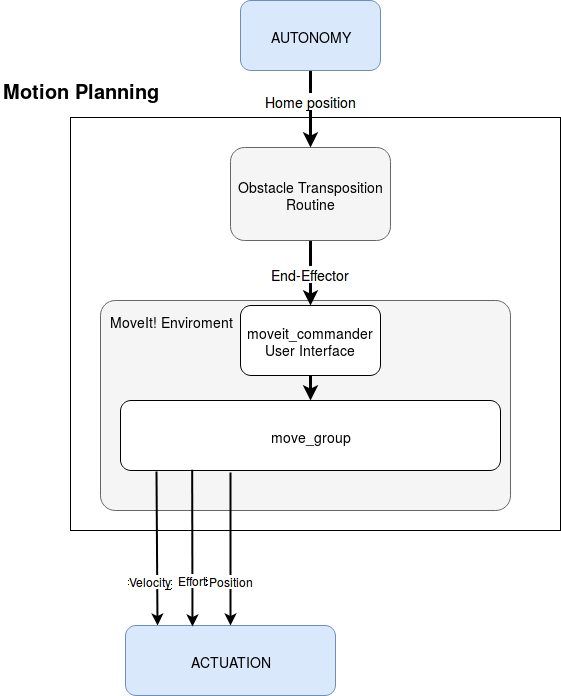
\includegraphics[width=0.8\textwidth]{motion_plan_func.png}
	\caption{Fluxograma de funcionamento da funcionalidade de Motion Planning}
	\label{fig:flux_motion}
	\source{Própria}
\end{figure}

\subsubsection{Saídas}
Por meio da compatibilização do \textit{MoveIt!} com o \textit{ROS}, a saída dessa funcionalidade são os comandos de velocidade, esforço e posição para cada junta do robô.

\subsection{Actuation }
\label{ssec:actu}
\subsubsection{Definição da funcionalidade}
A funcionalidade de Actuation tem como objetivo mover a estrutura física do robô, possibilitando o controle dos movimentos das juntas, garras e unidades de tração.
\subsubsection{Dependências}
Essa funcionalidade depende das funcionalidades de \textit{Power Management} e \textit{Motion Planning}. O \textit{Power Management} será responsável por fazer alimentação dos motores, possibilitando controlar a corrente máxima fornecida para cada grupo.
A dependência em relação à funcionalidade de \textit{Motion Planning} está atrelada principalmente com o software \textit{MoveIt!}, que ao receber um \textit{end-effector},realiza o cálculo de trajetória e envia os comandos de velocidade, esforço e posição para os controladores das juntas, garras e unidades de tração.

\subsubsection{Premissas Necessárias}
Para o correto funcionamento desse módulo, devem ser consideradas as seguintes premissas:
\begin{itemize}
	\item Os motores devem estar configurados de acordo com o padrão de ID determinado pela equipe, fazendo parte da mesma malha de controle;
	\item Os controladores das juntas,garras e unidades devem estar configurados de acordo com os comandos que serão recebidos pelo\textit{ MoveIt!};
	\item Os 3 grupos de motores estarão em malhas de alimentação de 12V individuais.
\end{itemize}
\subsubsection{Descrição da Funcionalidade}
O \textit{ROS} disponibiliza uma série de drivers para compatibilização dos motores dynamixel, possibilitando a criação de controladores específicos no seu ambiente. Serão criados os controladores referentes as juntas e unidades de tração do robô.Os controladores receberão comandos de \textit{velocity} e \textit{position} do \textit{MoveIt!} junto com os comandos para movimentar o robô na linha.
Após os comandos serem recebidos pelos controladores, eles serão enviados para o \textit{hardware} do robô, de acordo do padrão de comunicação dos motores, por meio de comunicação serial. 
\begin{figure}[h]
	\centering
	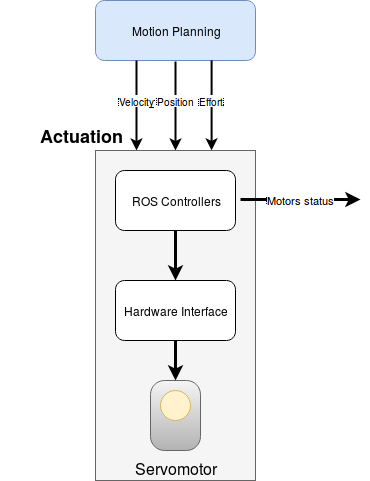
\includegraphics[width=0.6\textwidth]{actuation_depen.png}
	\caption{Fluxograma da funcionalidade Actuation}
	\label{fig:depen_actuation}
	\source{Própria}
\end{figure}
\subsubsection{Saídas}
A saída desta funcionalidade é o movimento da estrutura física do robô, que estará de acordo com o planejamento de trajetória do \textit{MoveIt!} e com as instruções para operação na linha

\subsection{Power Management}
\label{ssec:power}
\subsubsection{Definição da funcionalidade}

A funcionalidade de \textit{Power Management} é responsável pelo gerenciamento de alimentação elétrica dos componentes elétricos e eletrônicos do robô, através da integração das funcionalidades de seu firmware no ambiente \textit{ROS}.
\subsubsection{Dependências}
Essa funcionalidade depende da comunicação serial por meio da biblioteca \verb|rosserial| para compatibilização e integração das funcionalidades de firmware no ambiente \textit{ROS}. Operacionalização e customização do firmware embarcado no hardware de acordo com as necessidades do projeto e da alimentação fornecida pela placa multiplexadora, por meio de baterias Li-Ion NH2054 14.4 volts.

\subsubsection{Premissas Necessárias}
Para o correto funcionamento desse módulo de \textit{Power Management}, devem ser consideradas as seguintes premissas:
\begin{itemize}
	\item A placa multiplexadora estará conectada diretamente ao módulo de \textit{Power Management} 
	\item Todos os dispositivos estarão conectados nas suas respectivas entradas
	\item A placa deverá ser alimentada por 2 baterias de 14.4 Volts e 3 Amperes, totalizando um fornecimento de até 6 Amperes
	\item A placa estará conectada diretamente na NUC, por meio de uma USB	
	
\end{itemize}
\begin{figure}[h]
	\centering
	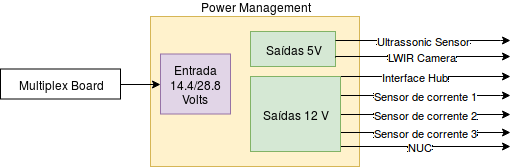
\includegraphics[width=1\textwidth]{power_management_hardware.png}
	\caption{Fluxograma de funcionamento da funcionalidade de Power Management}
	\label{fig:power_management_hardware}
	\source{Própria}
\end{figure}
\subsubsection{Descrição da Funcionalidade}
A funcionalidade \textit{Power Management} é responsável  fornece diversos recursos em sua totalidade. O hardware utilizado (placa Zord) possui um sensor de corrente e tensão para cada porta de saída, permitindo o monitoramento individual de cada uma das portas. O microcontrolador utilizado Atmega32U4 possui um firmware embarcado onde toda a compatibilização com o ambiente \textit{ROS} é realizada, o que torna essencial o uso do pacote rosserial para o seu funcionamento. O firmware é responsável pela ativação dos relés digitais em caso de surtos de corrente para proteção dos dispositivos elétricos. 
Os limites nos valores de corrente funcionam justamente para que o hardware interrompa a alimentação em um possível caso de surto de corrente. Todos os aspectos importantes para o funcionamento do sistema de gerenciamento de energia pode ser configurado tanto via \textit{ROS}, por meio das configurações dos serviços, ou por meio do firmware, modificando os parâmetros do tempo de duração dos picos de corrente. Os principais serviços e tópicos criados pela funcionalidade Power Management no \textit{ROS} são:
\begin{itemize}
	\item \textit{Tópicos}
	\begin{itemize}
		\item \textit{PowerOutput}
		Este tópico disponibiliza os valores de tensão e corrente de todas as portas da placa em tempo real.
		\item \textit{TakeStatus}
		Disponibiliza o estado de cada porta da placa, informando os eventos ocorridos e a porcentagem de corrente demandada durante a ocorrência do evento.
	\end{itemize} 
	\item \textit{Serviços} 
	\begin{itemize}
	\item \textit{GetCurrentLimitCommand}
	Este comando retorna o valor de corrente máxima de saída configurado para a porta escolhida
	\item \textit{SetCurrentLimitCommand}
	Este comando realiza a configuração do valor máximo de corrente de saída em uma determinada porta
	\item \textit{PowerOnOffCommand}
	Este comando realiza a ação de ativação ou desligamento de uma determinada porta.
	\end{itemize}
\end{itemize}
A placa de Gerenciamento de energia irá receber a carga das baterias pela placa multiplexadora e irá realiza o controle de alimentação dos seguintes componentes:
\begin{itemize}
	\item Grupos de servo motores
	\item Grupo de sensores de corrente
	\item NUC
	\item Interface HUB
	\item Câmera LWIR
	\item Sensor ultrassônico
	\item Phidgets
	\item STM Nucleo
	\item Módulo GPS
\end{itemize}

\subsubsection{Saídas}
A funcionalidade irá disponibilizar a energia para o robô e as seguintes estruturas no ambiente \textit{ROS}:
\begin{itemize}
	\item Tópicos com informações de tensão e corrente nas portas
	\item Tópico para aviso de sobre-corrente
	\item Tópico para informar disponibilidade da placa
	\item Serviços para ler e configurar limite de corrente das portas
	\item Serviço para ligar ou desligar energia em uma porta	
\end{itemize}

\subsection{System Integrity Check}
\label{ssec:check}

\subsubsection{Definição da funcionalidade}
É a funcionalidade responsável por checar a integridade do sistema antes do início da missão, verificando os subsistemas e suas variáveis.

\subsubsection{Dependências}
A funcionalidade receberá informações dos seguintes componentes
\begin{itemize}
	\item Sensor de Temperatura
	\item Servomotores
	\item Câmera IR
	\item Câmera Stéreo
	\item IMU
	\item Sensor de Proximidade
	\item Placa de Power Management
	\item Sonar 
	\item Baterias
\end{itemize}

Todas as informações serão enviadas por meio do ambiente \textit{ROS}, na forma de \textit{Services} ou \textit{Publishers}.

\subsubsection{Premissas Necessárias}
As premissas necessárias para o funcionamento dessa funcionalidade são:
\begin{itemize}
	\item Os subsistemas do robô irão disponibilizar o seu status no ambiente \textit{ROS} por meio de tópicos ou serviços
	\item A checagem fará parte do planejamento de missão
\end{itemize}

\subsubsection{Descrição da Funcionalidade}
A checagem da integridade do sistema é uma funcionalidade essencial para garantir o sucesso da missão e preservar a integridade do robô. O \textit{ROS} facilita essa comunicação entre os subsistemas, possibilitando que seja criada uma rotina de checagem antes de cada missão.

Será disponibilizado no sistema uma rotina para iniciar a missão. Ao receber o comando para início de missão, os sistemas serão checados sequencialmente, utilizando estrutura de \textit{Services} e \textit{Publishers} do \textit{ROS}. Caso algum sistema apresente falha, a missão não se iniciará e o erro será mostrado no \textit{terminal} e registrado no arquivo de \verb|log|. Se todos os sistemas estiverem em funcionamento, se iniciará a missão. O fluxograma da funcionalidade está ilustrado na figura \ref{fig:sys_check_flux}.	
\begin{figure}[h]
	\centering
	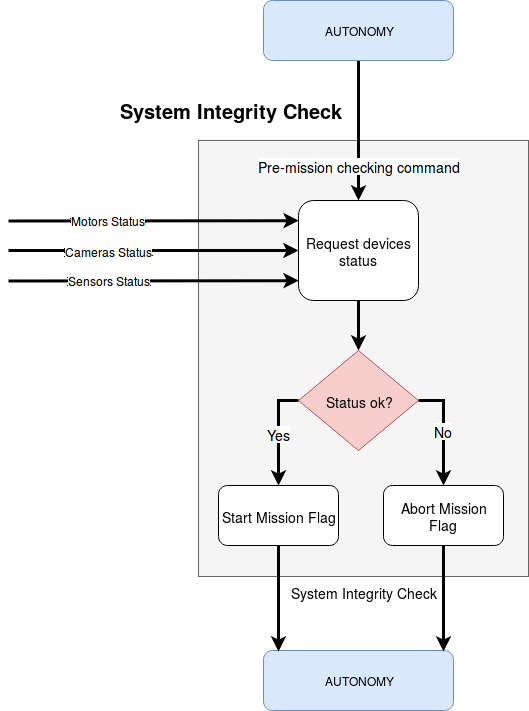
\includegraphics[width=0.6\textwidth]{sys_check_flux.png}
	\caption{Fluxograma da rotina para checagem do sistema}
	\label{fig:sys_check_flux}
	\source{Própria}
\end{figure} 


\subsubsection{Saídas}
No início da rotina de inspeção, a funcionalidade será responsável por enviar o sinal inicia a missão. Caso todos os sistemas checados estejam funcionando, a inspeção ocorrerá normalmente, se algum sistema apresentar defeitos, o defeito será mostrado no \textit{terminal}, registrado em log e a missão será abortada.


%--------- NEW SECTION ----------------------
\section{Simulação do sistema}
\label{sec:sim}
A simulação de sistemas robóticos consistem em um dos pilares para o desenvolvimento de projetos. Com a simulação é possível testar aplicações sem a necessidade de adquirir componentes, os membros da equipe de projeto conseguem trabalhar de forma simultânea no robô enquanto o protótipo físico fica reservado para testes específicos.

O \textit{ROS} oferece ferramentas de visualização já integradas no seu sistema, o RVIz, que possibilita o usuário visualizar os modelos do robô e também administrar plugins, como de mapeamento e planejamento de movimento, que é o caso do \textit{MoveIt!}.

Para a simulação do robô no ambiente aberto, é utilizado  o software \textit{Gazebo}. A integração entre \textit{ROS} e \textit{Gazebo} consegue fazer com que o modelo \textit{URDF}, por mais que não seja o nativo do \textit{Gazebo}, seja aceito na simulação. Parâmetros do mundo podem ser ajustados e a integração de plugins como câmeras e sensores faz com que a simulação consiga ser utilizada em diferentes estudos. Algoritmos de imagem podem ser testados com os plugins de câmera já implementados, proporcionando um auxílio para demonstrar conceitos e teorias de funcionamentos

A simulação fornecida possui os controladores de juntas já implementados, fazendo com que testes de códigos de movimentação e testes de controles já pudessem ser previamente testados, poupando riscos de dano ao protótipo e possibilitando trabalho simultâneo.

\begin{figure}[h!]												
	\centering												
	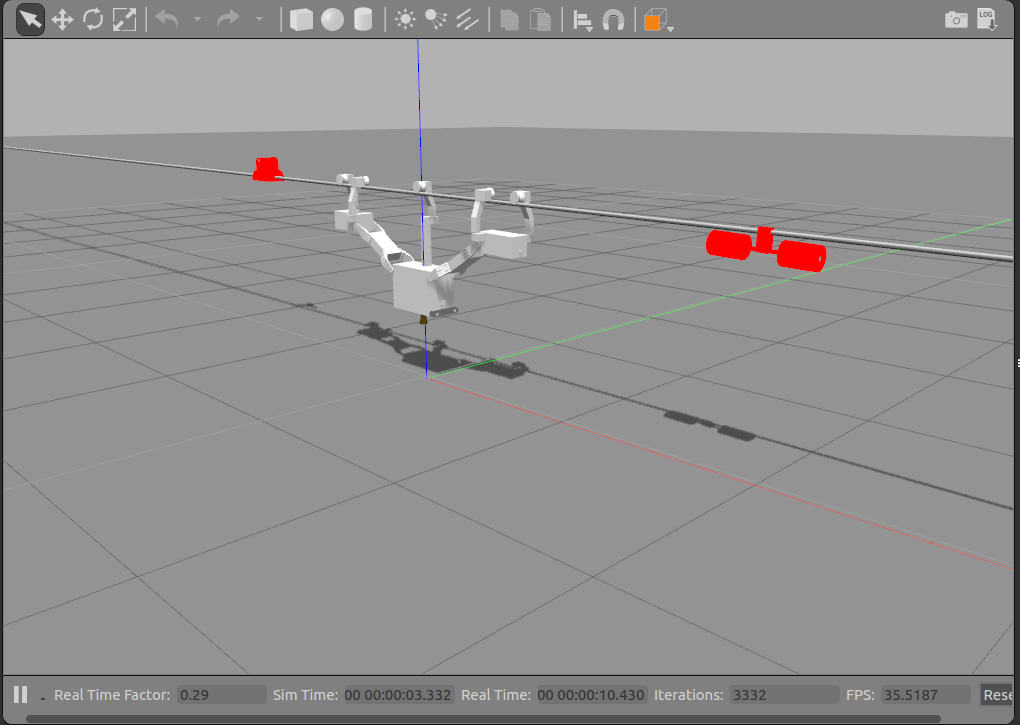
\includegraphics[width=0.6\textwidth]{elir_no_gazebo.png}				
	\caption{Simulação do \textit{ELIR} no \textit{Gazebo}.}		
	\label{img:gazebo1}									
\end{figure}

